\subsection{Spread across inputs and random starts}
\label{sec:spread}

\begin{figure}[tbp]
  \centering
  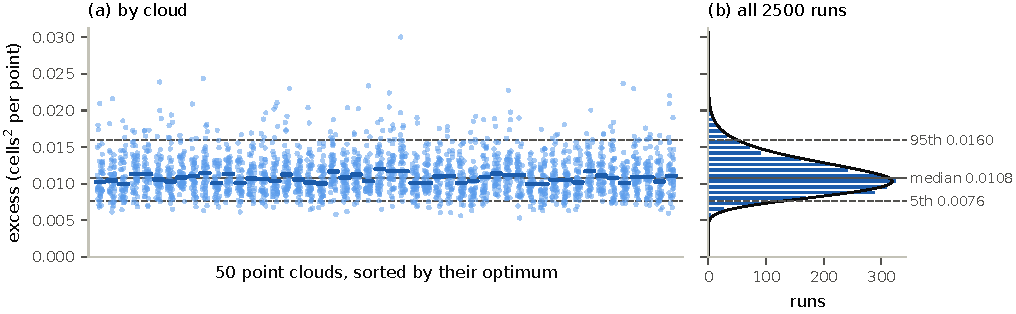
\includegraphics[width=\linewidth]{figures/fig_seed_study.pdf}
  \caption{Excess of the default preset over the optimum, in cells$^2$ per point, on 50 clouds
  of $10^4$ uniform points, each run from 50 random starts. (a)~Each column is one cloud, its
  dots are the 50 starts and its bar is their median; clouds are sorted by their optimum.
  (b)~All 2{,}500 runs, with a fitted log-normal curve. The solid line is the median, the
  dashed lines the 5th and 95th percentiles; every cloud spans about the same band.}
  \label{fig:spread}
\end{figure}

\begin{figure}[tbp]
  \centering
  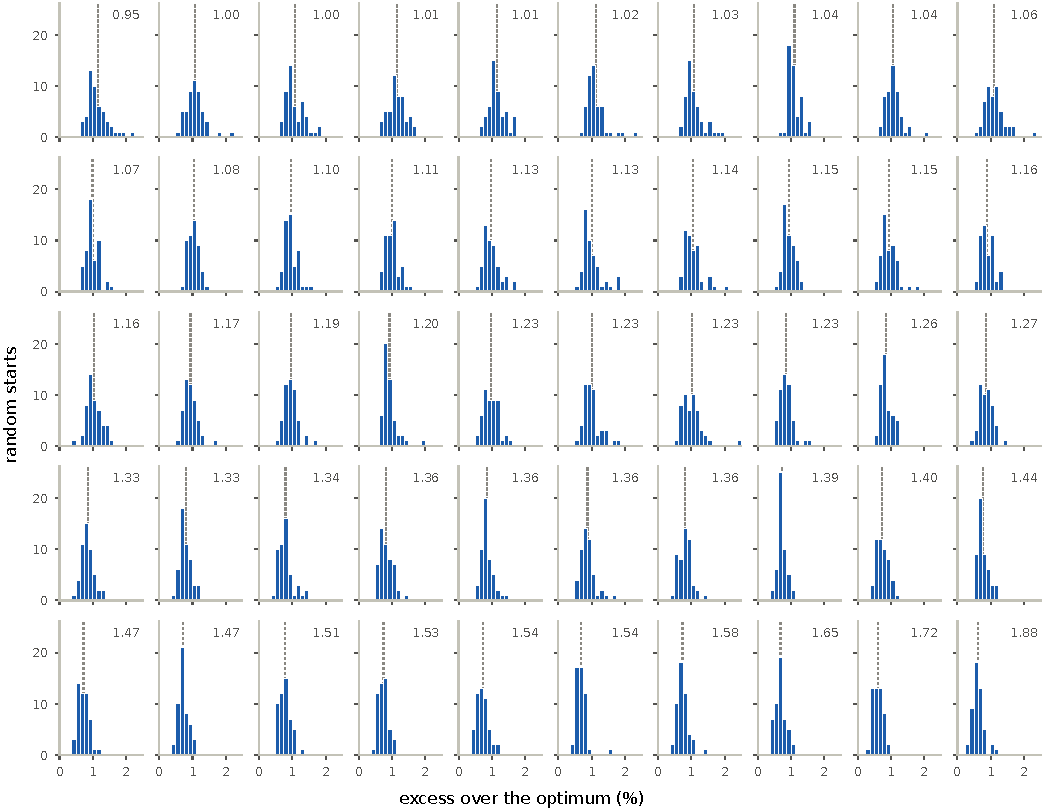
\includegraphics[width=\linewidth]{figures/fig_seed_hists.pdf}
  \caption{The runs of Figure~\ref{fig:spread}, one histogram per cloud over its 50 random
  starts, on shared axes. Clouds are sorted by their optimum, printed in each panel in
  cells$^2$ per point; the dashed line is the mean over the starts. The histograms keep the
  same width and shape from cloud to cloud and move left as the optimum grows, because the
  absolute excess stays about the same.}
  \label{fig:spread-hists}
\end{figure}

The constructed fixed point shows how bad a fixed point can be, but it starts from a
layout that the method never chooses. To see how much the result depends on the input and
on the random start in practice, we drew 50 clouds of $10^4$ uniform points (instance seeds
100--149, used nowhere else), the hardest common input, and ran the default preset from 50
random starts on each (method seeds 0--49), 2{,}500 runs in all. Each cloud's optimum came
from dense SciPy. In addition, the certified solver, warm-started from each of the 2{,}500
\ShuffleSnap\ layouts, reached the same optimum every time.

From a random start, the result is a draw from one distribution, and that distribution is
nearly the same for every cloud. Measured in absolute terms, as cells$^2$ per point added to
the optimum, 96\% of the variance comes from the start and 4\% from the cloud
(Figure~\ref{fig:spread}a); only 7 of the 50 clouds' distributions differ from the pooled one
at the 5\% level, where 2.5 would by chance. The distribution is right-skewed rather than
normal: within a cloud the skewness is 0.93, 31 of 50 clouds fail a Shapiro--Wilk test, and
23 runs lie more than three standard deviations above their cloud's mean, where a normal
distribution would put 3.4. On a log scale it is close to normal (skewness 0.28, 5 of 50
clouds fail the test). The pooled runs fit a log-normal distribution with a median of
0.0109\,cells$^2$ per point and $\sigma=0.23$ (Figure~\ref{fig:spread}b), and 90\% of runs
fall between 0.71 and 1.48 times that median.

In relative terms, the excess had a mean of 0.91\% (standard deviation 0.26\%) and a median
of 0.87\%, and 90\% of runs fell between 0.55\% and 1.38\%. The extremes were 0.32\% and
2.44\%. Even the worst run left 75\% of its points on their optimal cells (82\% on average).
Because the absolute excess hardly depends on the cloud while the optimum varies by a factor
of two (0.95--1.88\,cells$^2$ per point), clouds with a larger optimum show a smaller
relative excess: the correlation between a cloud's optimum and its mean relative excess is
$-0.94$, and $-0.04$ for the absolute excess. Each cloud's histogram of relative excess
therefore has the same shape and moves left as its optimum grows
(Figure~\ref{fig:spread-hists}). The start accounts for 67\% of the variance of the relative
excess; on one cloud, the 50 starts span a median of 0.99 percentage points.

For a user, one run at this size is a sample from a known, narrow distribution. Keeping the
best of several starts helps less than a larger window: the best of 2, 4 and 10 starts
averages 0.79\%, 0.72\% and 0.65\%, while the quality preset reaches 0.28\% at about three
times the default's time (Table~\ref{tab:main10k}). The constructed fixed point, whose relative excess is unbounded, lies
far outside this distribution. This is evidence, not a bound: it covers one size and one
distribution, and on uniform points the excess grows with $N$ (Section~\ref{sec:scaling}).
